%% Los cap'itulos inician con \chapter{T'itulo}, estos aparecen numerados y
%% se incluyen en el 'indice general.
%%
%% Recuerda que aqu'i ya puedes escribir acentos como: 'a, 'e, 'i, etc.
%% La letra n con tilde es: 'n.

\chapter{Evaluaci\'on}
\section{Sistema de Visi\'on}
Se ha hecho pruebas con el sistema de visi\'on el cual encuentra los c\'irculos de las marcas sobre los robots, esto es realizado con la transformada de Hough.
\begin{figure}
	\centering
	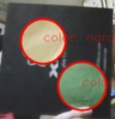
\includegraphics[width=2.5in]{imagen7.jpg}
	
	\caption{Ubicacion de los circulos}
	\label{fig_mar}
\end{figure}

Desp\'ues podemos calcular la posicion actual del robot, con los m\'etodos explicados en la propuesta.
\begin{figure}
	\centering
	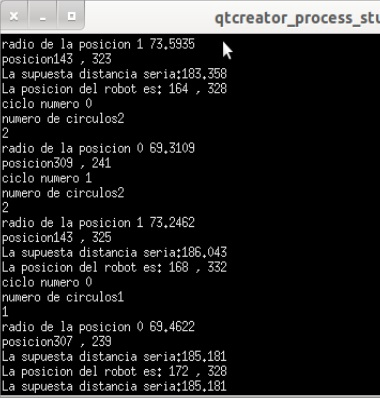
\includegraphics[width=2.5in]{imagen8.jpg}
	
	\caption{C\'alculo de la posici\'on actual del robot y la orientaci\'on}
	\label{fig_mar}
\end{figure}